\chapter{Experiments}

\section{Classical Computer Vision-based Approach}

\subsection{Gaze Projection}
\begin{figure}
    \centering
    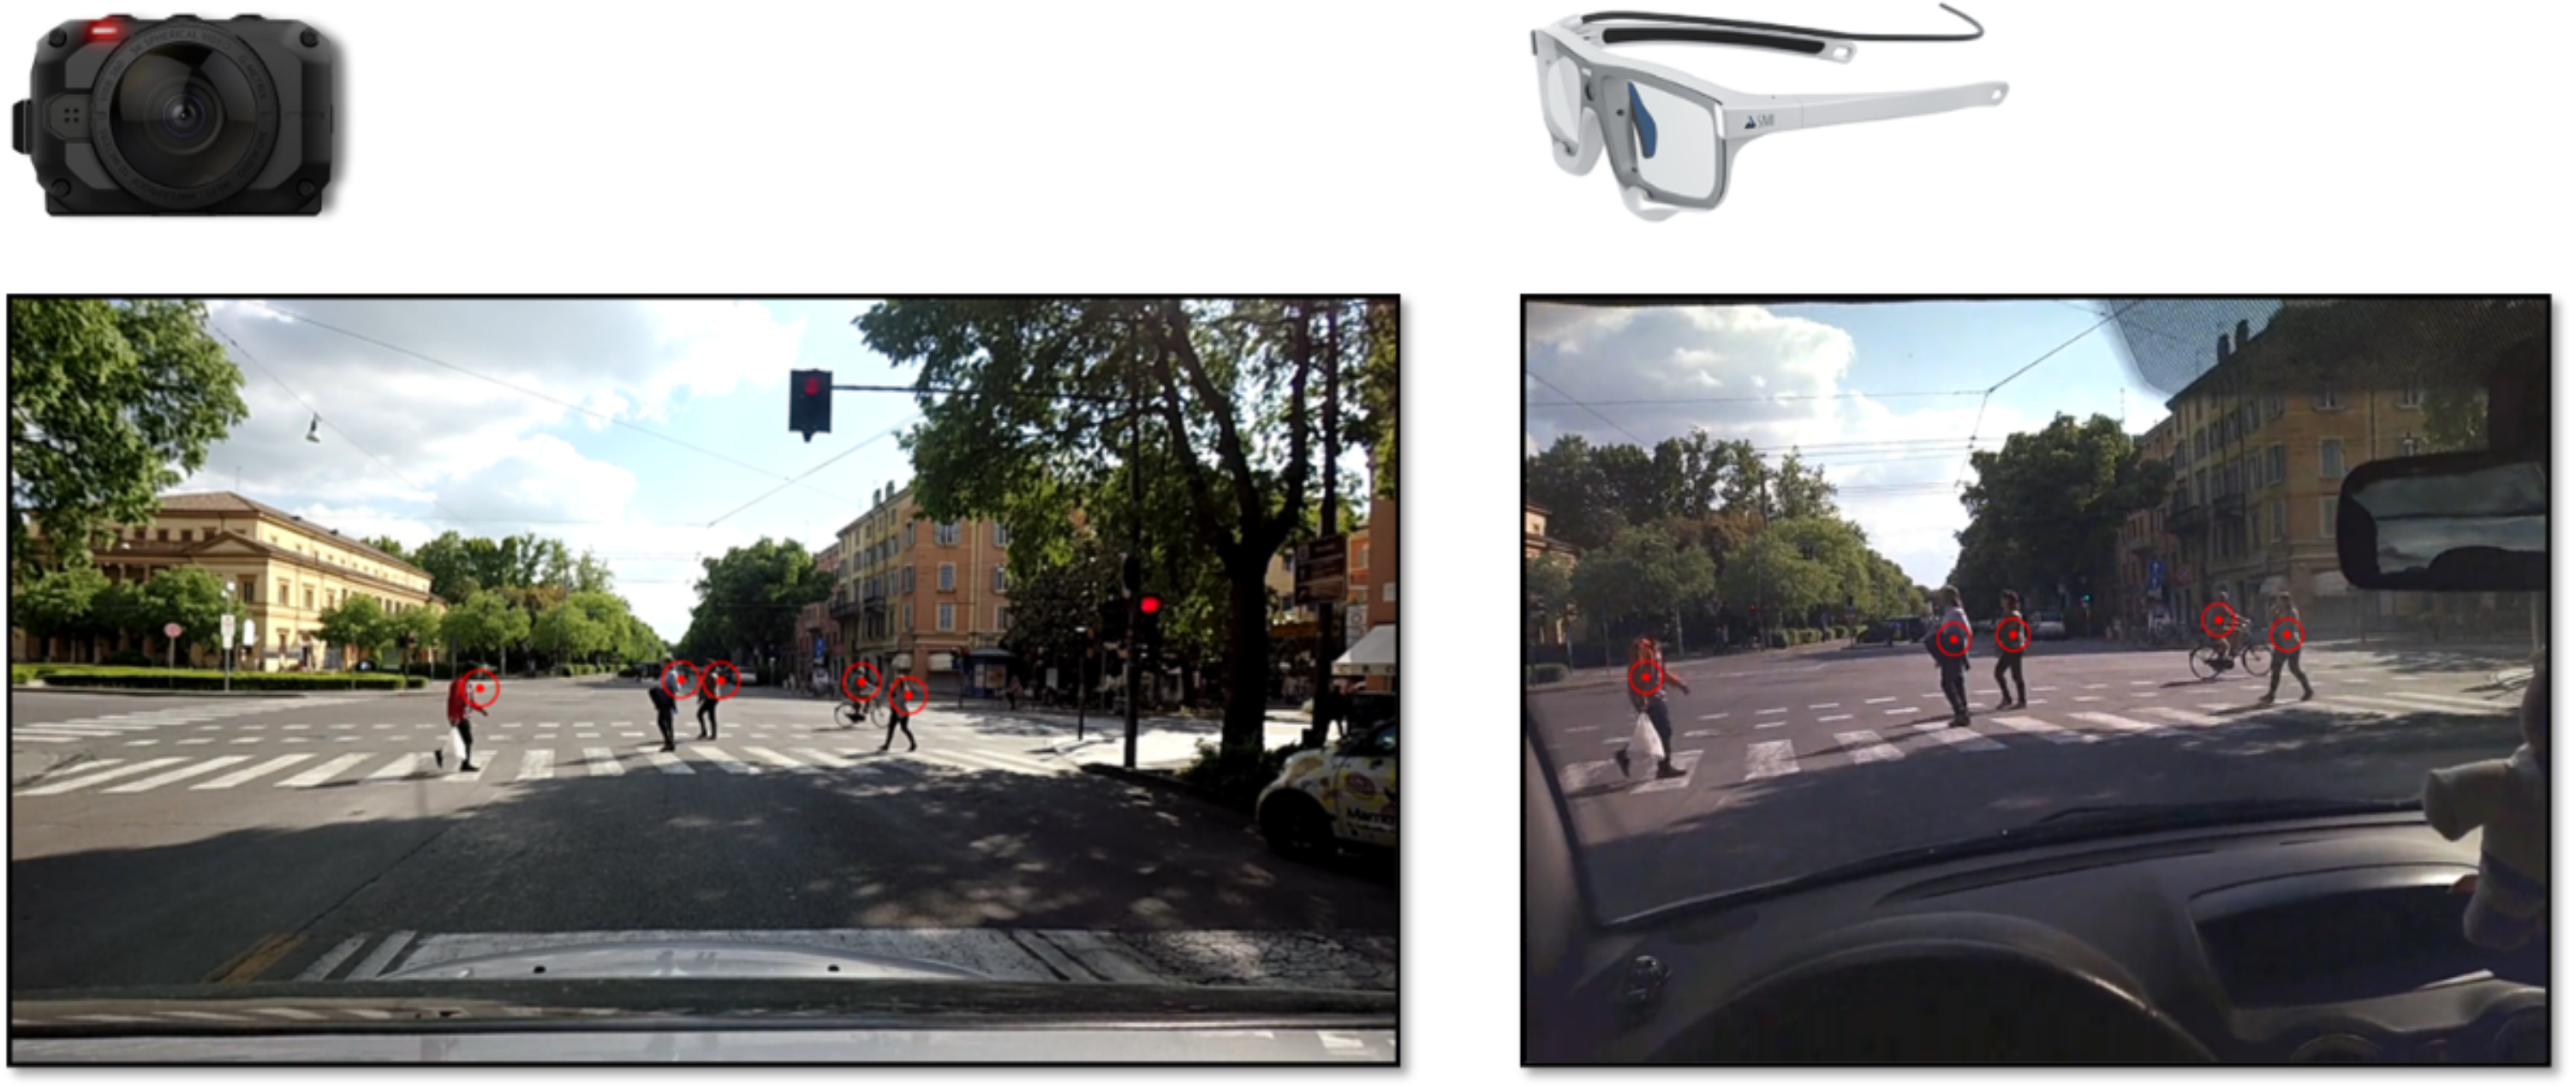
\includegraphics[width=\textwidth]{images/dreyeve/gaze_projection.png}
    \caption{Projection of the gaze from the ETG camera to the RT camera. 
    All the gaze points are manually set.
    \textbf{Left}: Roof top camera view.
    \textbf{Right}: ETG camera view.}
    \label{fig:gaze_projection}
\end{figure}
\begin{figure}
    \centering
    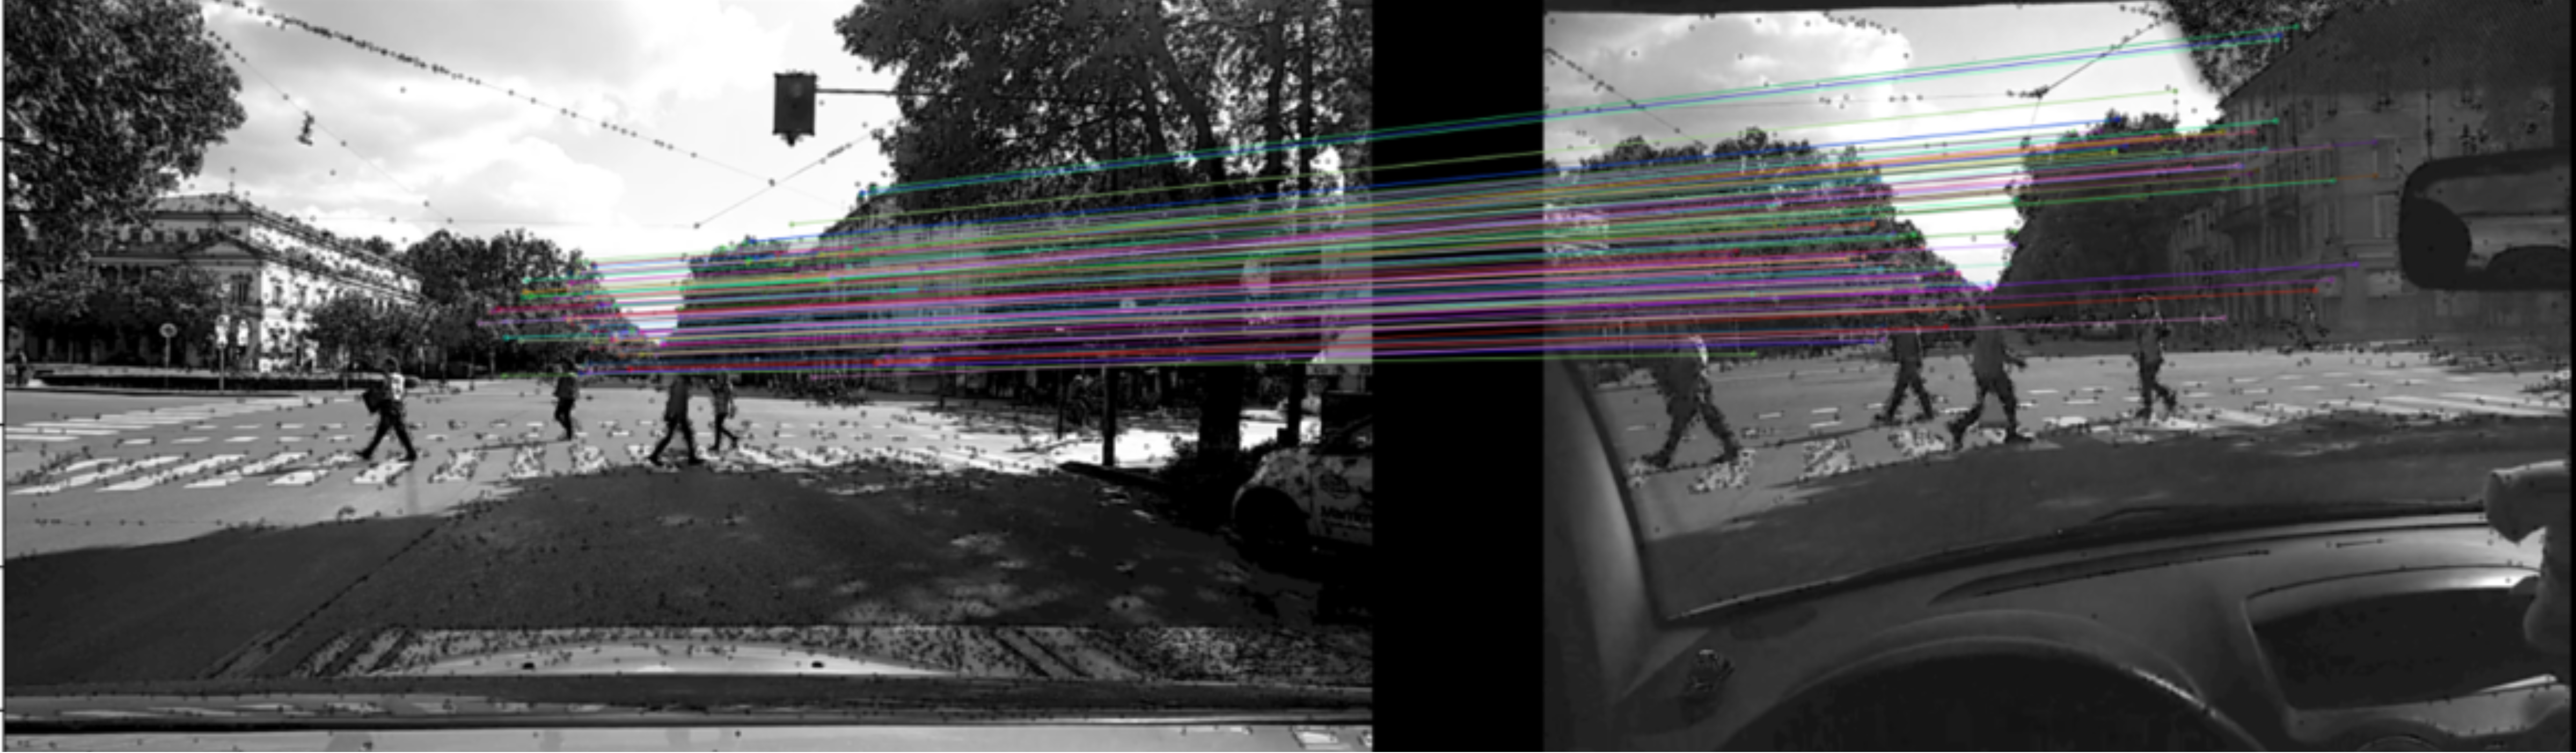
\includegraphics[width=\textwidth]{images/dreyeve/gaze_matchings.png}
    \caption{Projection of the gaze from the ETG camera to the RT camera. 
    All the gaze points are manually set.
    \textbf{Left}: Roof top camera view.
    \textbf{Right}: ETG camera view.}
    \label{fig:gaze_matchings}
\end{figure}
The projection of the gaze from the ETG camera to the RT camera is shown in 
Figure \ref{fig:gaze_projection}. We manually set some gaze points on the 
ETG camera such that they overlap with the vulnerable users. In this way, 
we are setting some operation points that we can use to evaluate the quality 
of the homography estimation. From the figure it is possible to see that the 
projection is not perfect, but it is a good approximation of the gaze in the 
RT camera plane. The small errors are due to the fact that the scene is not 
flat and the homography is a planar transformation. However, most pixels with 
high contrast correspond to objects that are far away from the vehicle, 
therefore the approximation is reasonable.

In Figure \ref{fig:gaze_matchings} we show keypoints' matchings between the 
two images. The keypoints are extracted using the SIFT algorithm.
In a first instance, matchings are computed according to the Lowe's ratio test, 
with a threshold of 0.7. This is to make sure that there is enough Euclidean 
distance from the best matching to the second best matching. Then, we apply 
the RANSAC algorithm, with a threshold of 5 pixels for the reprojection error.
Finally, we compute the homography matrix using the inliers from the RANSAC 
algorithm. To optimize the estimation problem, we set the maximum number of 
iterations to 2000 and a confidence of 99.5\%.

As it is possible to see from Figure \ref{fig:gaze_matchings}, the matchings 
are accurate enough to compute homography. The dark points are all the keypoints 
extracted with SIFT, and the colored lines are the correspondent matchings 
obtained through RANSAC. 
As expected, in a scenario wehre there is a high contrast between the road 
evironment and the sky, the matchings are related to those loactions. 
However, many other keypoints where there is high contrast are detected, for 
example on crosswalks, pedestrians and buildings. They are probably not matched 
beacuse they are not unique enough to satisfy the Lowe's ratio test.

This is a fundamental aspect to consider when designing a system that should be 
used in many different scenarios, during the day and night, in different weather 
conditions, etc. Moreover, in Figure \ref{fig:gaze_projection} and 
\ref{fig:gaze_matchings} we show the results of an especially favorable scenario, 
where there are good conditions of light and contrast, and the driver is looking 
straight ahead.

\subsection{Distribution of People in Dr(eye)ve}
After computing all the projected gaze points, we can focus on the interaction 
of the driver with the vulnerable users. Therefore, it is important to have 
a general overview of the distribution of people in the Dr(eye)ve dataset.
However, considering that the focus is on the interaction \emph{during time},
it is also important to embed poeple's tracking information in the analysis.

Therefore, in Figure \ref{fig:tracking_distribution} we count the number of 
different people that are tracked by the driver. In particular, on the lower 
x-axis there is the total observation time of the person in seconds. On the 
upper x-axis there is the number of frames where the person is tracked, this is 
just to have a different representation of the same data that considers 
preprocessing. On the y-axis there is the number of people observed by the driver 
for the specific amount of time. The distribution is shown in a logarithmic scale 
to better compare the values.
The plots also compare the downtown with all other scenarios. Green bars 
represent the downtown scenarios, while red bars represent the sum of all 
the scenarios in the dataset (therefore including the downtown).

The distribution is right-skewed, with a long tail of people that are observed 
for a short amount of time. 
On one hand, this is expected, considering that the driver is usually looking 
straight ahead when driving. On the other hand, it is important to consider 
that some missing data could be due to tracking losses or occlusions with 
ByteTrack, or some non-accurate gaze projections that do not overlap with the 
bounding boxes of the people.

In Figure \ref{fig:tracking_cum_distribution} we show the cumulative distribution 
of the tracking counts. This is a useful representation to understand the number 
of people that are observed for at least a certain amount of time. The plot

% Need to format the figures in a better way (increase font size)
\begin{figure}
    \centering
    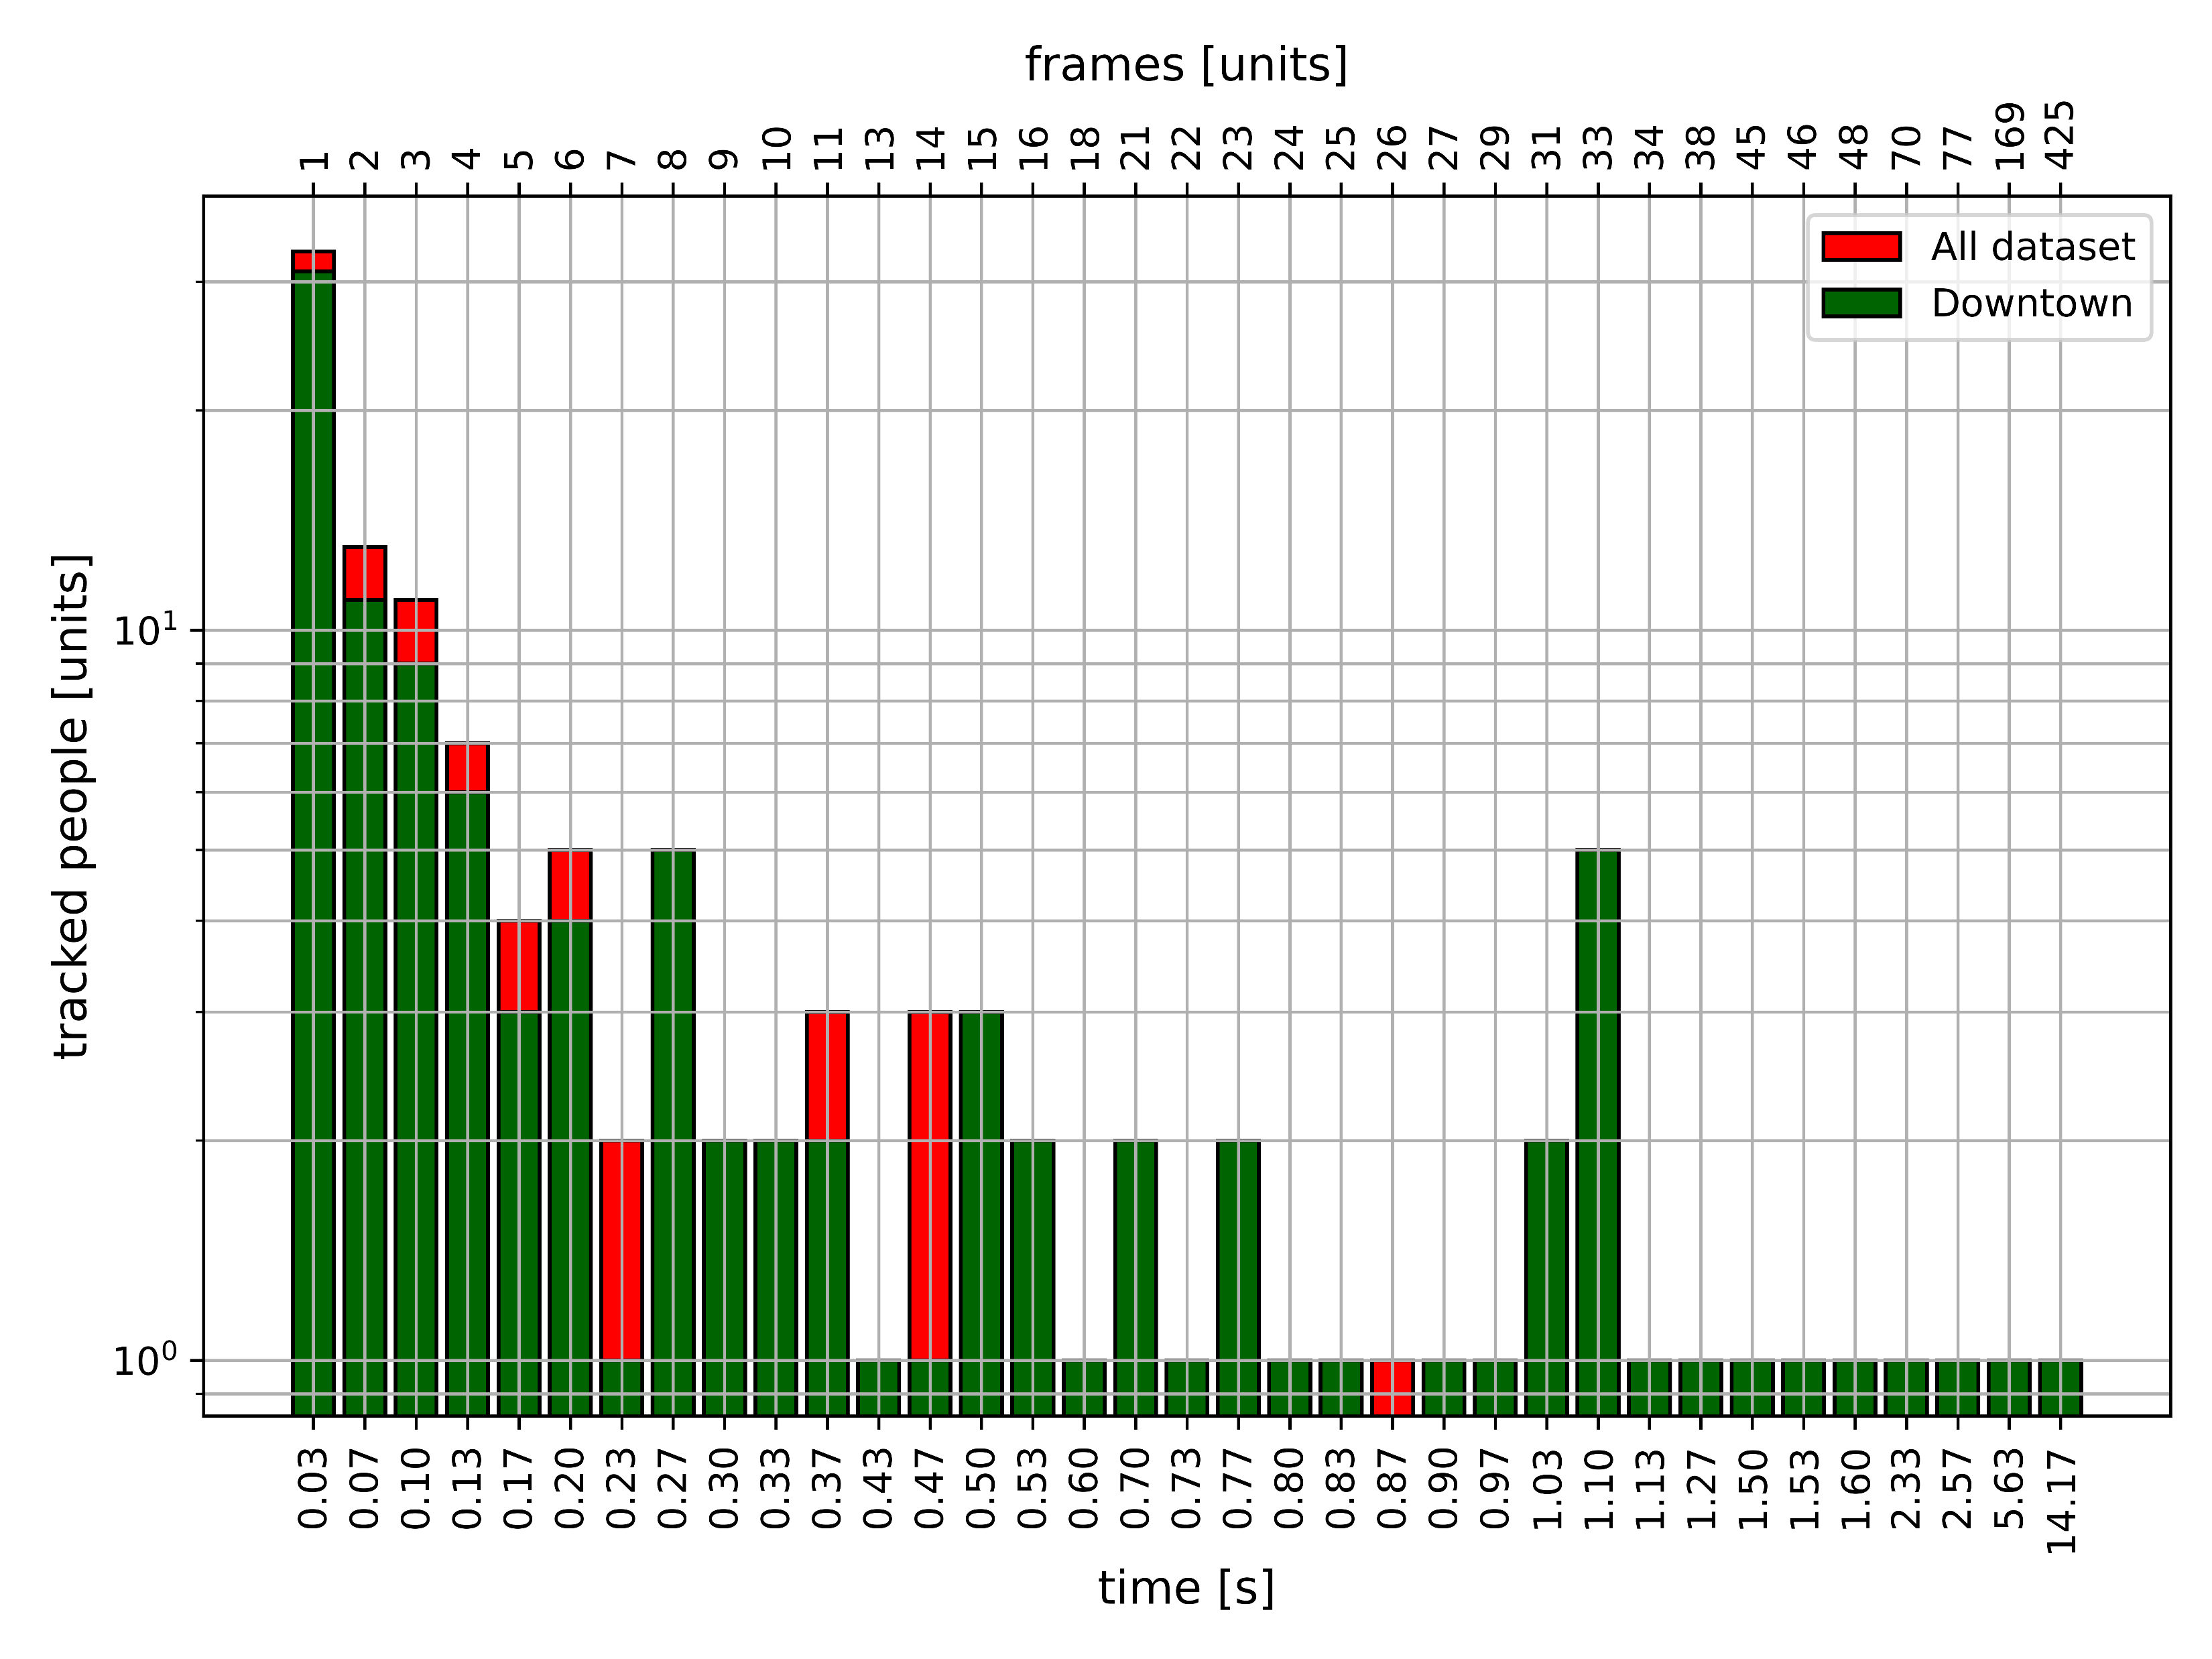
\includegraphics[width=0.9\textwidth]{images/dreyeve/tracking_distrib.png}
    \caption{Gaze tracking counts towards people in the Dr(eye)ve dataset.}
    \label{fig:tracking_distribution}
\end{figure}
\begin{figure}
    \centering
    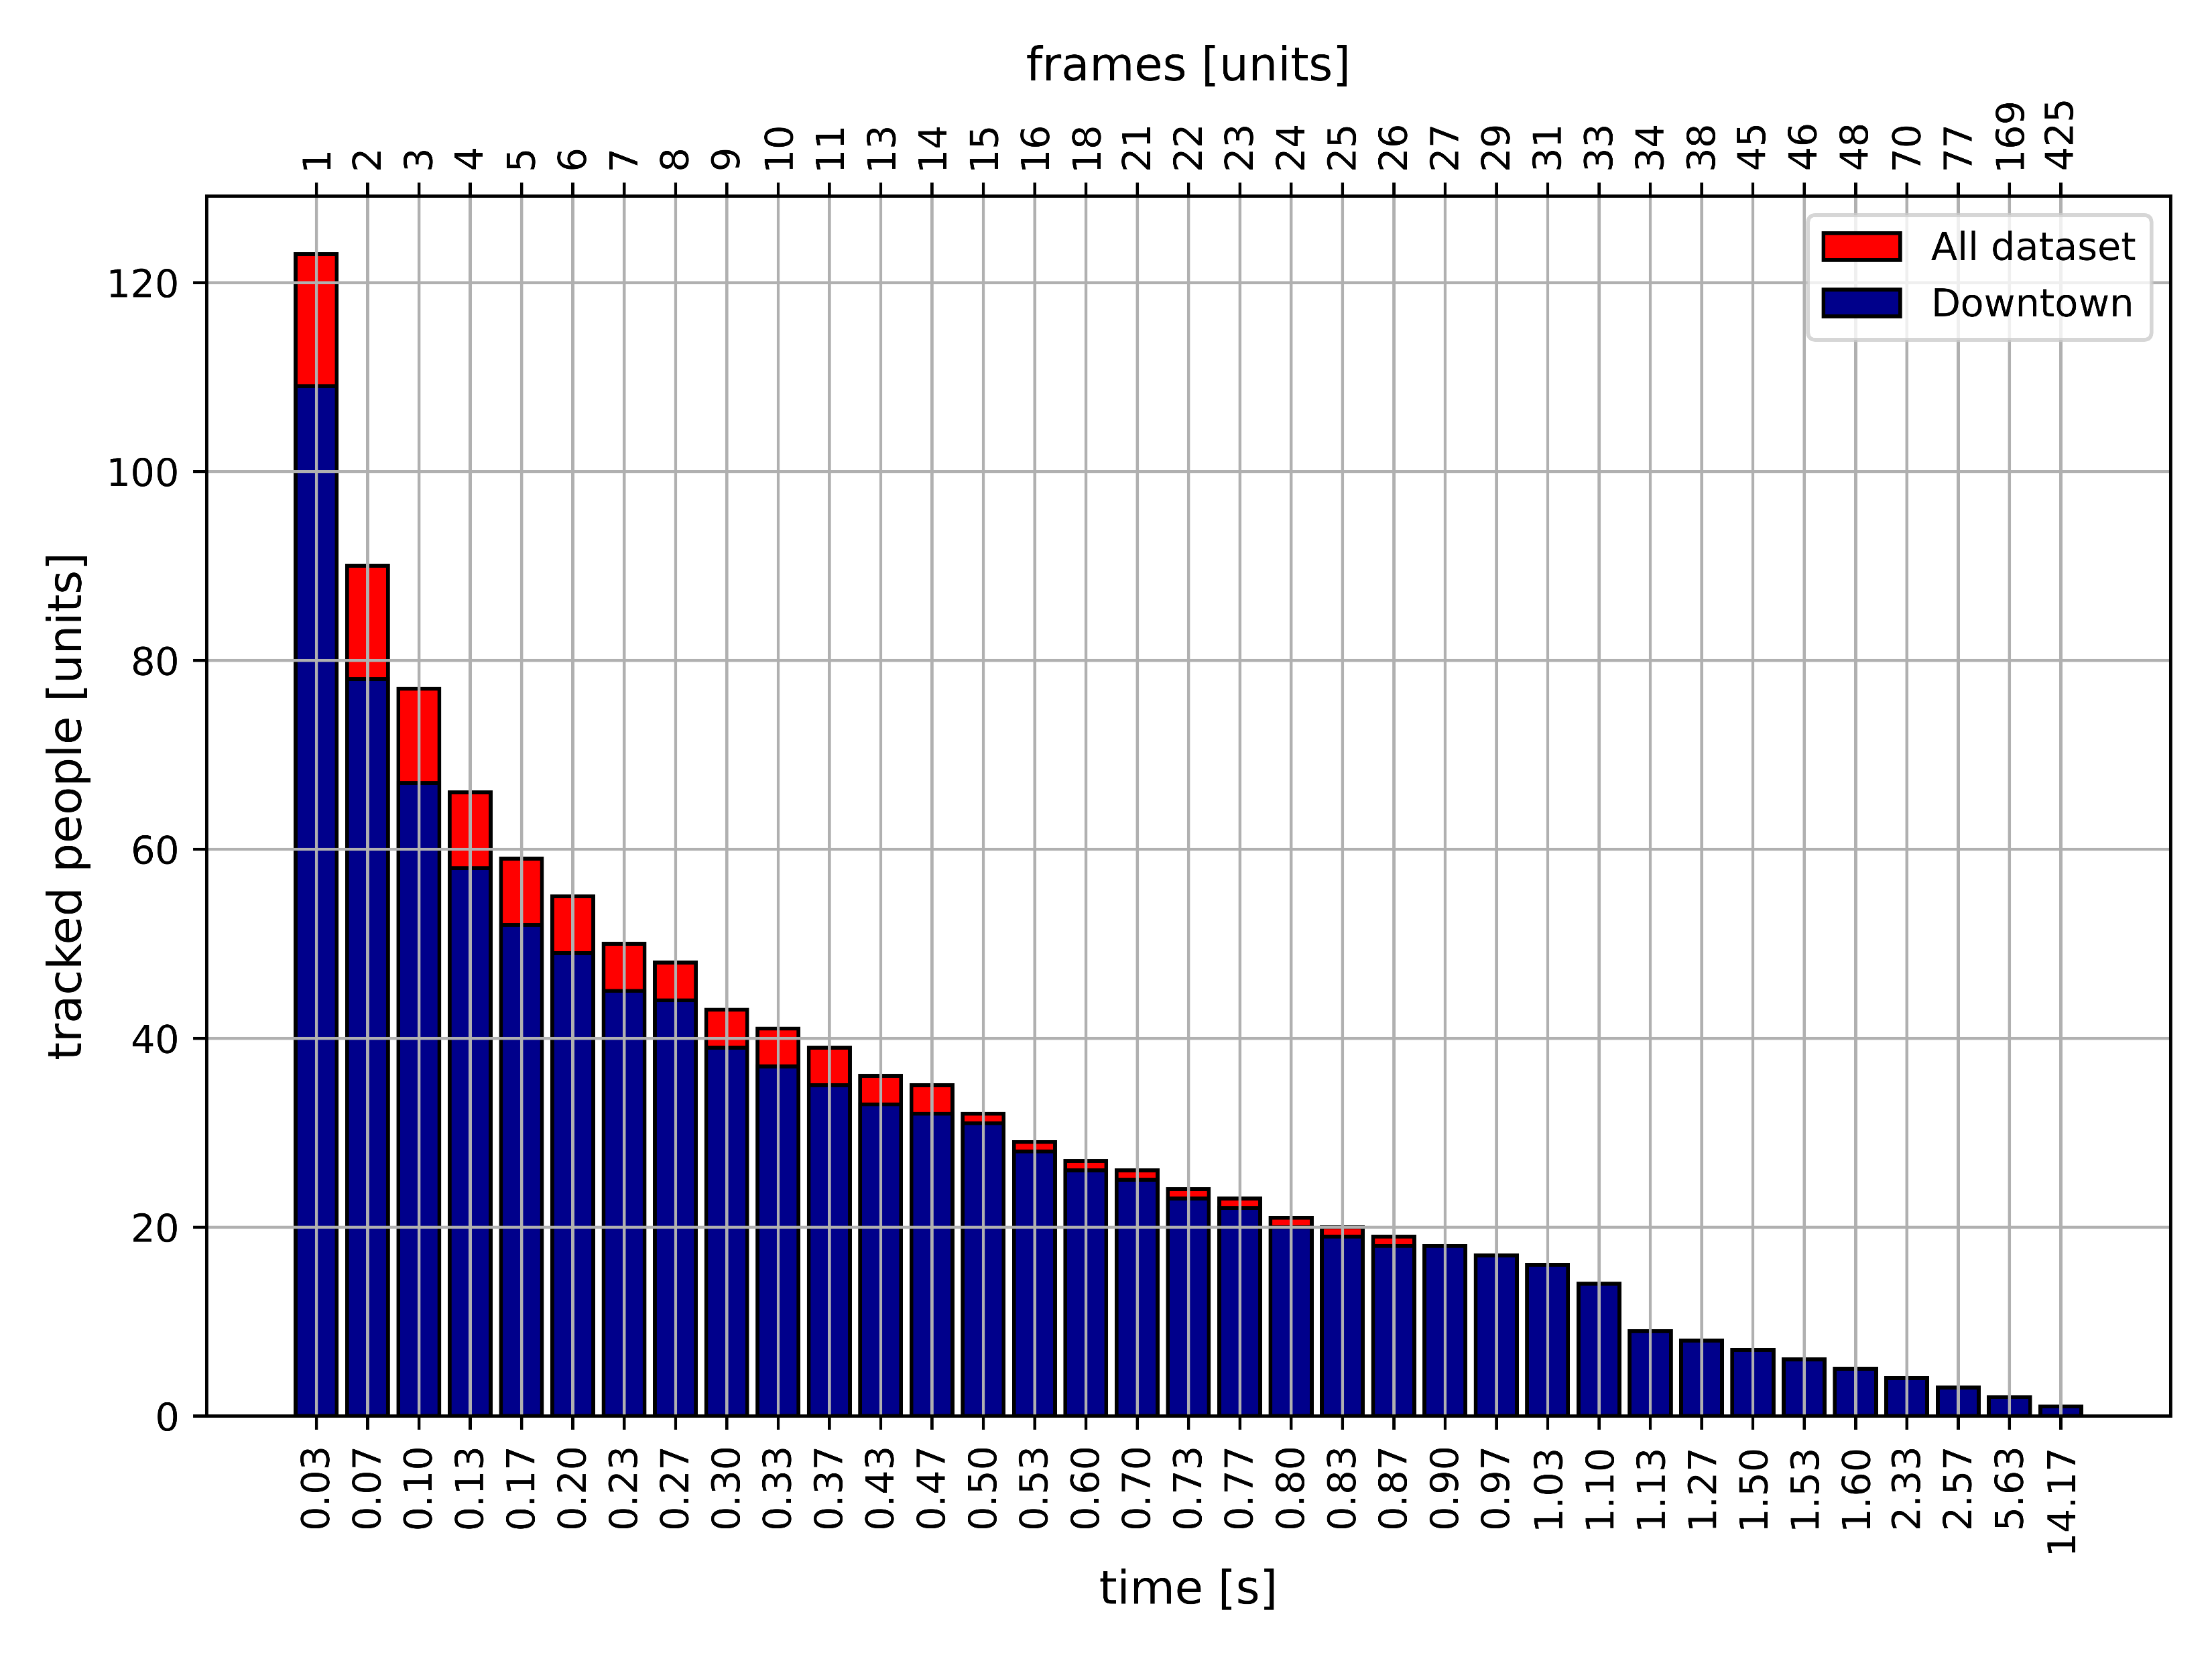
\includegraphics[width=0.9\textwidth]{images/dreyeve/tracking_distrib_cum.png}
    \caption{Cumulative distribution of gaze tracking counts in the Dr(eye)ve dataset.}
    \label{fig:tracking_cum_distribution}
\end{figure}

\subsection{Gaze Interaction with Targets}
\subsection{Adding Depth Information}

\section {Deep Learning-based Approach}
\subsection {Data Distribution of BDD100k}
\subsection{Supervised Training on Dr(eye)ve}
\subsection{Semi-Supervised Training on Dr(eye)ve}
\subsection{Supervised Training on BDD100k}
\subsection{Semi-Supervised Training on BDD100k}

\subsection{Experiments with GPT4-o}
In May 2024 OpenAI released GPT4-o, their multilingual, multimodal generative 
pre-trained transformer. Considering its powerful capability to describe general 
contexts in wide scenes, we decided to test the architecture to solve a problem 
similar to ours. Experiments were conducted on BDD100k dataset.

\subsubsection{Problem Definition}
We defined two groups of six images each. The first group consists of general 
driving scenarios that contain at least one person in each image. 
The second group, on the other hand, is still related to driving scenarios but 
does not contain any person. However, in most images of both groups there are 
some common objects, including cars, buildings, etc.
Then the model will be asked to evaluate a new, never seen, image and answer 
in which group it belongs.

Other experiments in the two groups were done, including asking the model which 
common targets are present in each group.

\subsubsection{Data Selections}
\setlength{\subfigwidth}{45mm}
\setlength{\horspace}{.3\textwidth}
\begin{figure}
    \centering
    \begin{tabular}{p{\horspace} p{\horspace} p{\horspace}}
    \begin{subfigure}[b]{\subfigwidth}
        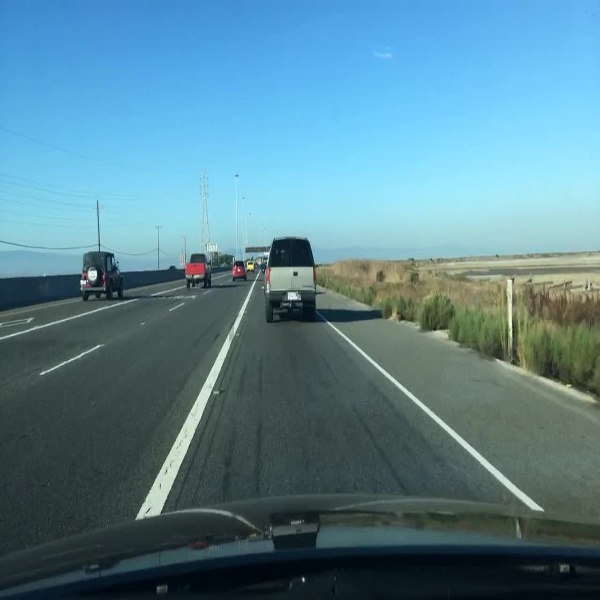
\includegraphics[width=\subfigwidth]{images/gpt4/s1.jpg}
    \end{subfigure}
    \hfill &
    \begin{subfigure}[b]{\subfigwidth}
        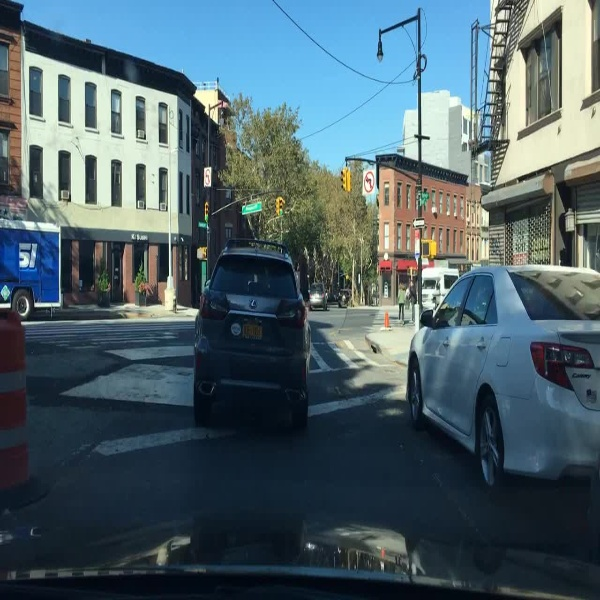
\includegraphics[width=\subfigwidth]{images/gpt4/s2.jpg}
    \end{subfigure} 
    \hfill &
    \begin{subfigure}[b]{\subfigwidth}
        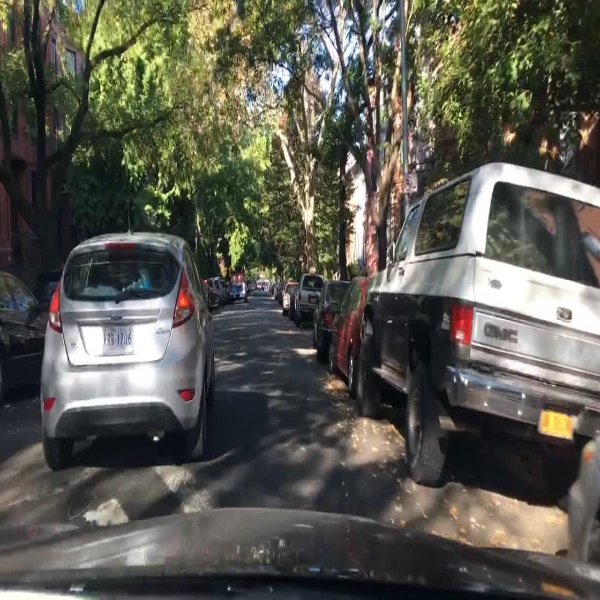
\includegraphics[width=\subfigwidth]{images/gpt4/s3.jpg}
    \end{subfigure} \\
    %
    \begin{subfigure}[b]{\subfigwidth}
        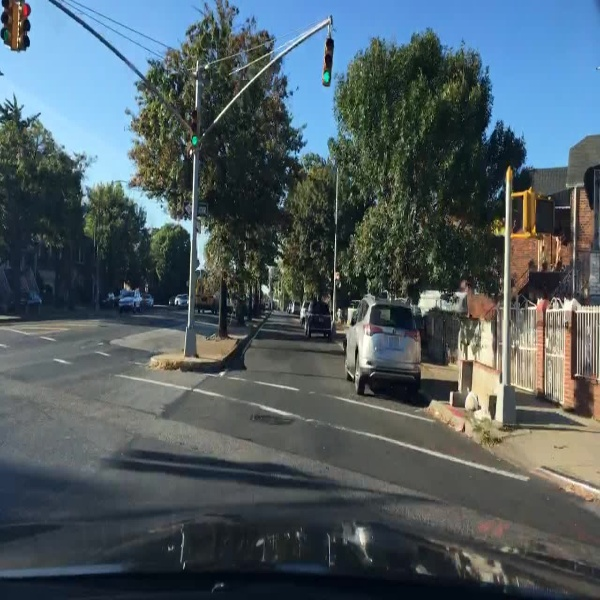
\includegraphics[width=\subfigwidth]{images/gpt4/s4.jpg}
    \end{subfigure}
    \hfill &
    \begin{subfigure}[b]{\subfigwidth}
        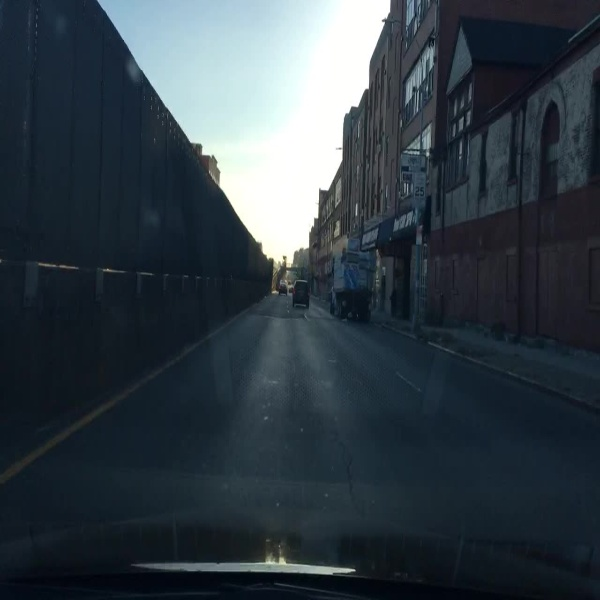
\includegraphics[width=\subfigwidth]{images/gpt4/s5.jpg}
    \end{subfigure} 
    \hfill &
    \begin{subfigure}[b]{\subfigwidth}
        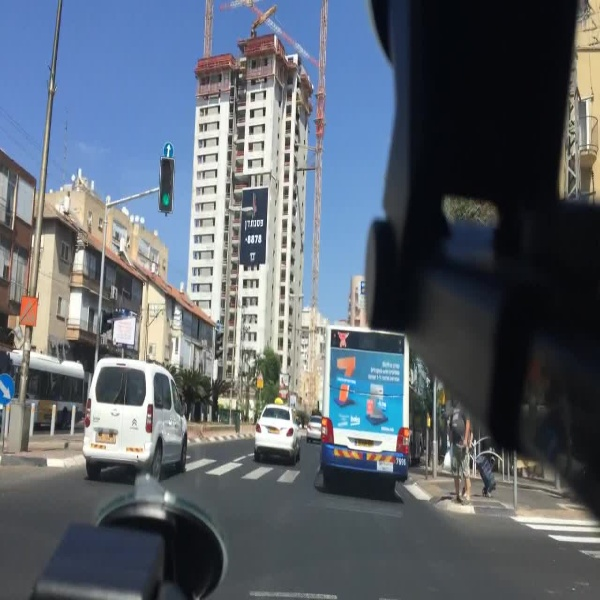
\includegraphics[width=\subfigwidth]{images/gpt4/s6.jpg}
    \end{subfigure}
\end{tabular}
\caption{Group of safe images, there are no people in all the images.}
\label{fig:safe_group}
\end{figure}
%
\begin{figure}
    \centering
    \begin{tabular}{p{\horspace} p{\horspace} p{\horspace}}
    \begin{subfigure}[b]{\subfigwidth}
        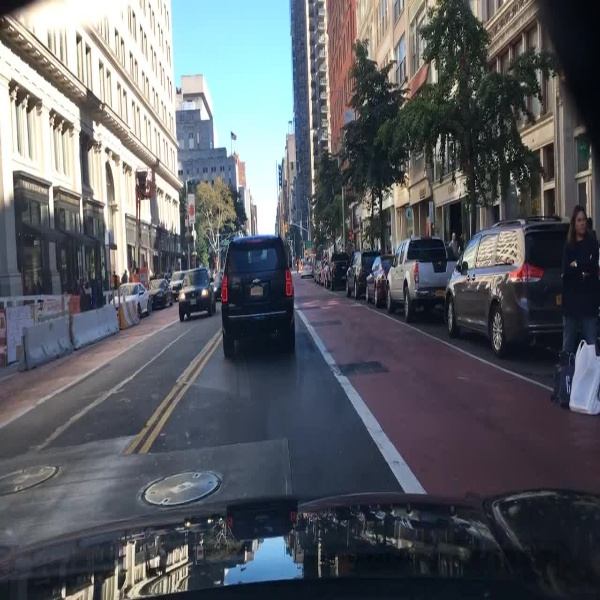
\includegraphics[width=\subfigwidth]{images/gpt4/d1.jpg}
    \end{subfigure}
    \hfill &
    \begin{subfigure}[b]{\subfigwidth}
        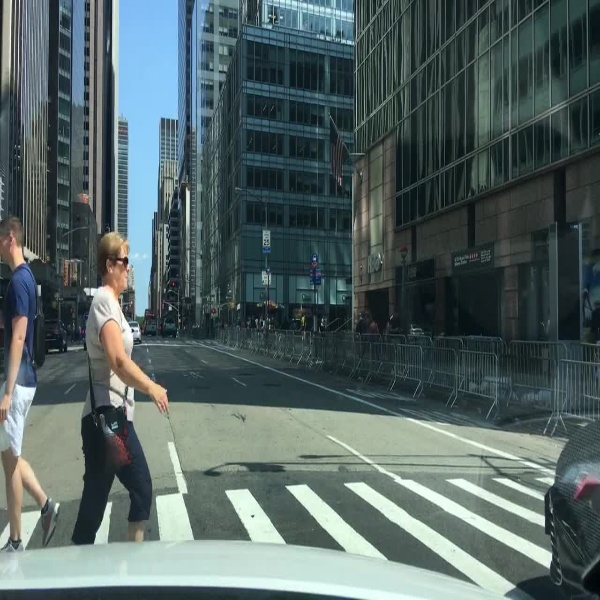
\includegraphics[width=\subfigwidth]{images/gpt4/d2.jpg}
    \end{subfigure} 
    \hfill &
    \begin{subfigure}[b]{\subfigwidth}
        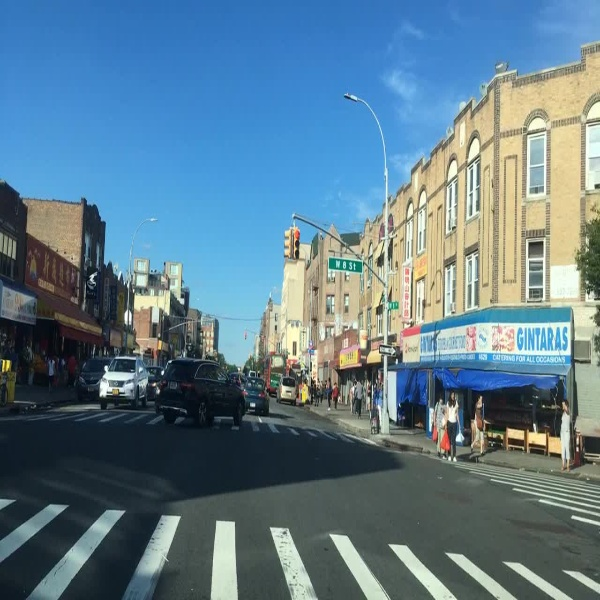
\includegraphics[width=\subfigwidth]{images/gpt4/d3.jpg}
    \end{subfigure} \\
    %
    \begin{subfigure}[b]{\subfigwidth}
        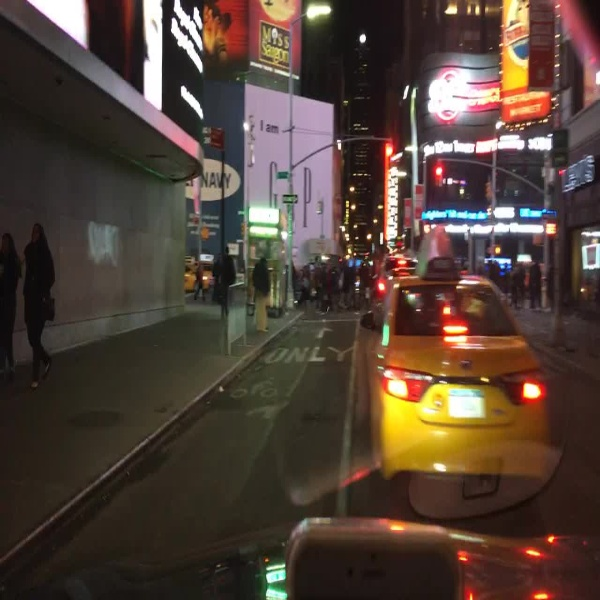
\includegraphics[width=\subfigwidth]{images/gpt4/d4.jpg}
    \end{subfigure}
    \hfill &
    \begin{subfigure}[b]{\subfigwidth}
        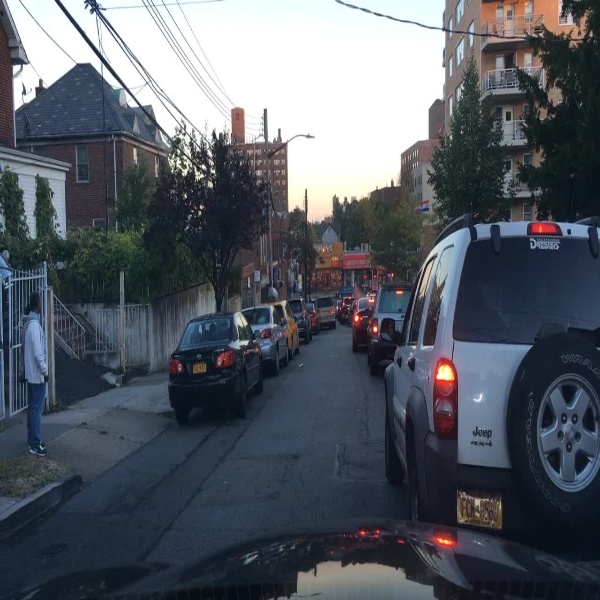
\includegraphics[width=\subfigwidth]{images/gpt4/d5.jpg}
    \end{subfigure} 
    \hfill &
    \begin{subfigure}[b]{\subfigwidth}
        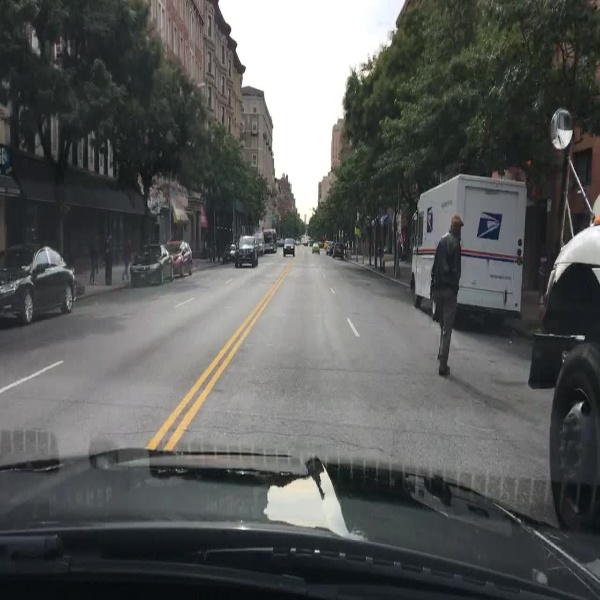
\includegraphics[width=\subfigwidth]{images/gpt4/d6.jpg}
    \end{subfigure}
\end{tabular}
\caption{Group of dangerous images, there are some people in each image.}
\label{fig:dangerous_group}
\end{figure}
The first group of images is shown in Figure \ref{fig:safe_group}. It consists 
of six images that do not contain any person. In particular, in the first image 
on the top left there is the ego-vehicle in a highway with some other vehicles 
on the front. The second on the top-center represents a downtown scenario with 
some vehicles on the front. In the third image on top-right there is a vehicle 
on the front and many vehicles parked on both sides of the road. The fourth 
image on bottom-left represents the ego-vehicle driving on a road with a traffic 
divider and some cars parked on the right side. In the fifth image on the 
bottom-center there is a straight road with some vehicles on the front and tall 
buildings on the sides. The last image on the bottom-right represents a 
downtown scenario with some vehicles, including cars and a bus. There is 
actually an occluded person in the image, but it is almost not visible.

The second group of images is shown in Figure \ref{fig:dangerous_group}. 
In the first image on the top-left there are two cars in fron of the ego-vehicle, 
some cars parked on both sides and a pedestrian standing on the right side. There 
are also some other pedestrians far away on sidewalks, not much visible in the 
image.
The second image on the top-center represents a downtown scenario where some 
pedestrians are crossing the road. There is also a car partially visible on the 
right of the ego-vehicle. The environment is characterized by tall buildings.
The third image on the top-right represents a downtown scenario with some 
empty crosswalks but many pedestrians on sidewalks. There are also some cars 
driving on the main road.
The fourth image on the bottom-left represents a night downtown scenario with a 
taxi in front of the ego-vehicle and group of pedestrians on the left sidewalk 
and far away, where there are crosswalks and red traffic lights.
In the fifth image, bottom-center, there is a line of cars in front of the 
ego-vehicle, some cars parked on the left side, and a pedestrian standing on the 
left sidewalk.
The last image on the bottom-right represents a main road with some vehicles 
parked on both sides, some others driving, and a person standing on the right 
side of the road.

Considering the dangerous scenarios, some specific cases were carefully selected,
especially with people partially visible, in the corners of the images, and 
on the background. On the other hand, in both groups there are many vehicles, both 
in foreground and background, that contribute to add noise to the data to 
classify.
This decision represents a further challenge for the model to 
isolate the right group of pixels.

\subsubsection{Common Features Extraction}
The first experiment consists of showing the model the two groups of images, 
without explicitly explaining the difference between them. The model is asked 
to describe the common targets in each group. The question-answer pairs are 
shown below:
%
{\fontfamily{cmr}\selectfont
\begin{description}
    \item[Q:] What common targets do all the images have?
    Do not list a target if it is not inside all the images. 
    (\emph{showing the dangerous images})
    \item[A:] Cars, roads, \hl{people}, sky.
    \item[Q:] What common targets do all the images have?
    Do not list a target if it is not inside all the images. 
    (\emph{showing the safe images})
    \item[A:] Road, \hl{other vehicles}, sorrounding environment.    
\end{description}
}
It is possible to notice that for the dangerous images the model correctly 
detects also people as common targets. Moreover, vehicles are shown in both 
groups, and the model is able to distinguish them as common targets correctly.
This means that the model is able to extract the common noise in both groups 
(the presence of cars, that usually occupy many pixels with respect to people), 
but at the same time it is able to extract features of people related to the 
dangerous group.

This is a promising result, considering that GPT4 is a pretrained model on 
general multimodal data, and not specifically on driving scenarios. 
However, it has over 174 billion parameters, and that is why it is capable to 
generalize in many different contexts. Using a vision transformer architecture 
for specific tasks, like driving scenarios, with much less parameters, could 
still lead to good results.

\subsubsection{Grouping and Classification}
\setlength{\subfigwidth}{45mm}
\setlength{\horspace}{.3\textwidth}
\begin{figure}
    \centering
    \begin{tabular}{p{\horspace} p{\horspace}}
    \begin{subfigure}[b]{\subfigwidth}
        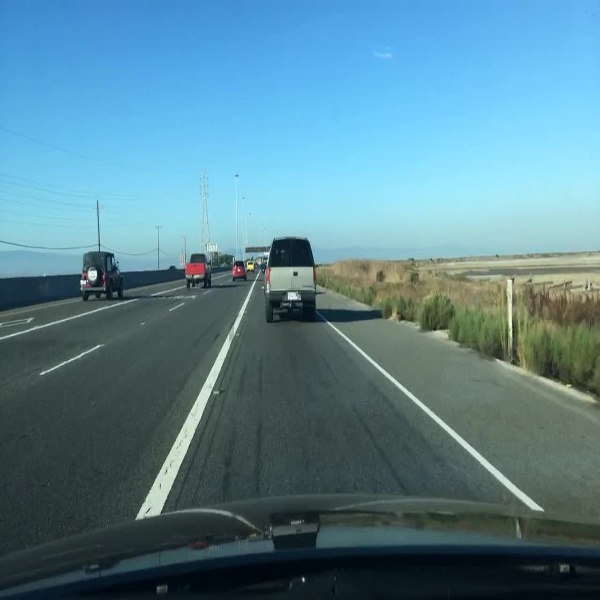
\includegraphics[width=\subfigwidth]{images/gpt4/s1.jpg}
    \end{subfigure}
    \hfill &
    \begin{subfigure}[b]{\subfigwidth}
        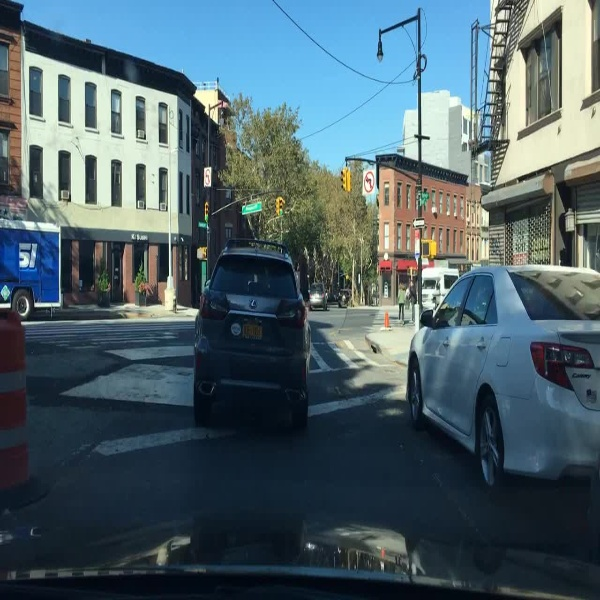
\includegraphics[width=\subfigwidth]{images/gpt4/s2.jpg}
    \end{subfigure} \\
    %
    \begin{subfigure}[b]{\subfigwidth}
        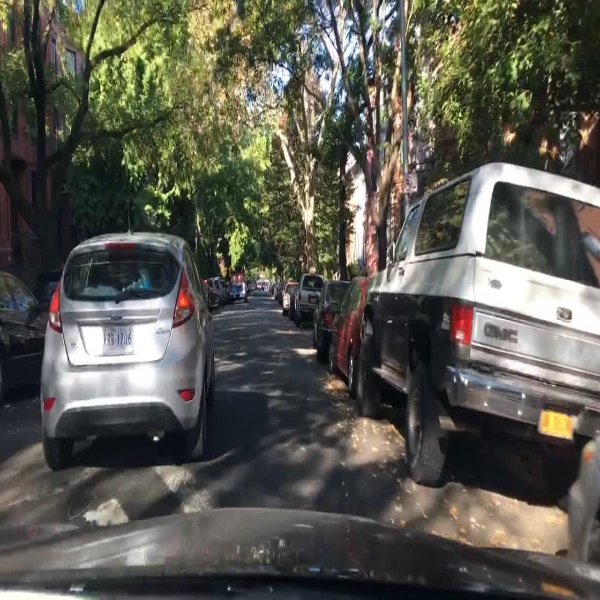
\includegraphics[width=\subfigwidth]{images/gpt4/s3.jpg}
    \end{subfigure}
    \hfill &
    \begin{subfigure}[b]{\subfigwidth}
        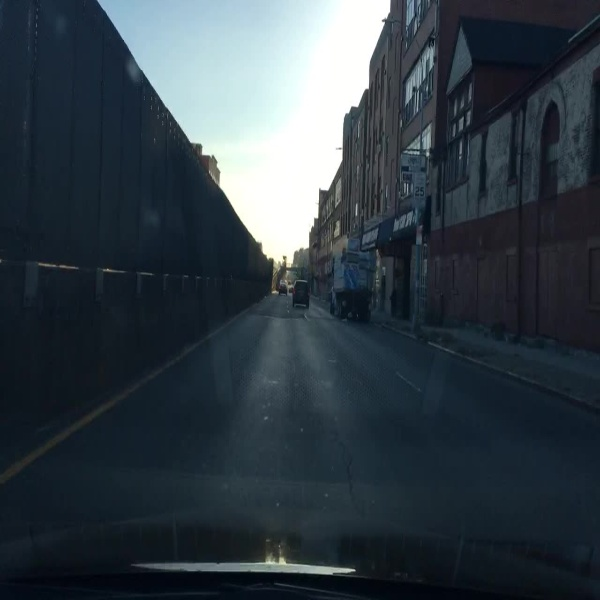
\includegraphics[width=\subfigwidth]{images/gpt4/s5.jpg}
    \end{subfigure}
\end{tabular}
\caption{Group of safe images, there are no people in all the images.}
\label{fig:sub_dangerous_group}
\end{figure}
%
\begin{figure}
    \centering
    \begin{tabular}{p{\horspace} p{\horspace}}
    \begin{subfigure}[b]{\subfigwidth}
        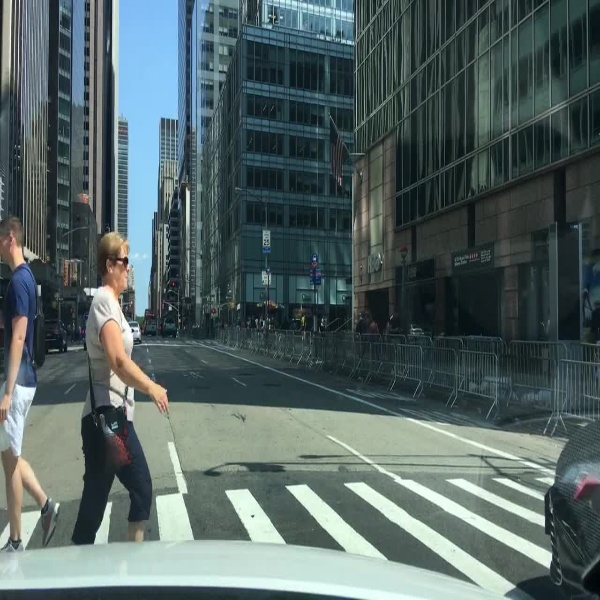
\includegraphics[width=\subfigwidth]{images/gpt4/d2.jpg}
    \end{subfigure}
    \hfill &
    \begin{subfigure}[b]{\subfigwidth}
        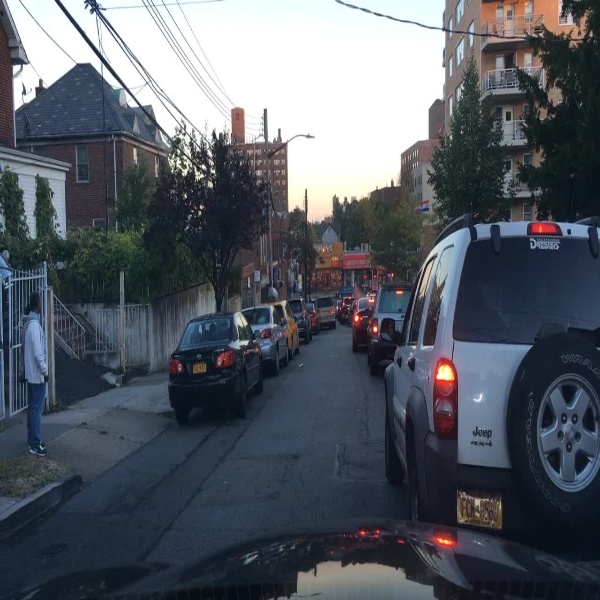
\includegraphics[width=\subfigwidth]{images/gpt4/d5.jpg}
    \end{subfigure} \\
    %
    \begin{subfigure}[b]{\subfigwidth}
        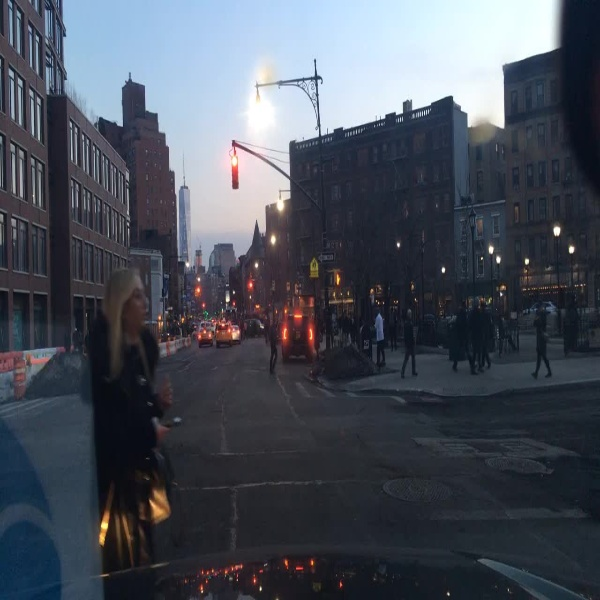
\includegraphics[width=\subfigwidth]{images/gpt4/d7.jpg}
    \end{subfigure}
    \hfill &
    \begin{subfigure}[b]{\subfigwidth}
        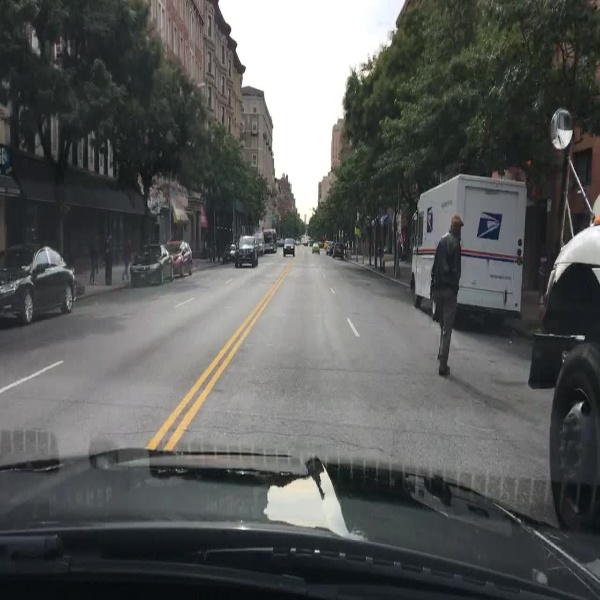
\includegraphics[width=\subfigwidth]{images/gpt4/d6.jpg}
    \end{subfigure}
\end{tabular}
\caption{Group of safe images, there are no people in all the images.}
\label{fig:sub_safe_group}
\end{figure}
\begin{figure}
\centering
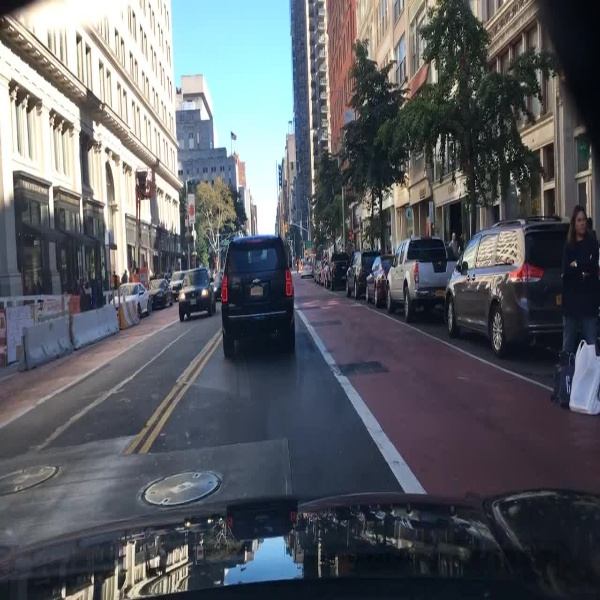
\includegraphics[width=\subfigwidth]{images/gpt4/d1.jpg}
\caption{Test image}
\label{fig:test_image}
\end{figure}

In this experiment we only showed the model the two groups of images, without 
asking to extract common targets. Then we show a new image and ask the model 
to classify it in the right group. The question-answer pairs are shown below:
{\fontfamily{cmr}\selectfont
\begin{description}
    \item[Q:] I will show you two groups of images. Then I will show you a test 
    image and you have to tell me what group it is related to. You have to 
    identify common features for each group to find the correct matching. Do not 
    output anything before I have finished, when I will tell you "predict this 
    image".
    \item[A:] Understood! I'm ready when you are to proceed with the image groups 
    and the test image.
    \item[Q:] This is the first group. (\emph{showing the first group of images})
    \item[A:] I've received the first group of images. Please show me the next group.
    \item[Q:] This is the second group. (\emph{showing the second group of images})
    \item[A:] I've received the second group of images. Please proceed with showing 
    the test image when you are ready.
    \item[Q:] This is the test image. (\emph{showing the test image})
    \item[A:] Based on the test image and comparing it to the two groups shown earlier:
    The test image features an urban setting with buildings lining the streets 
    and multiple vehicles on the road. It closely resembles the environment and 
    context of the images in the second group, which also depict urban settings 
    with buildings, streets, and a 
    \hl{visible presence of pedestrians} or traffic. 
    This environment is distinct from the first group, which primarily showed 
    roads in more open, less densely populated areas or showing less urban 
    characteristics. 
    Therefore, \hl{the test image belongs to the second group}.
\end{description}
}
Also in this experiment the model is able to correctly classify the test image 
in the right group. The model is able to give a detailed explanation of the 
features that are common in the test image and in the second group of images.
It is impressive that the model is capable to give such detailed explanations 
of contexts in images, considering that it is a general model and not specifically 
trained on driving scenarios.
